\chapter{Asking Luxury Shoppers How They Got RICH! (Dallas)}

This chapter is best read as a field lecture on wealth rather than a classroom derivation. We begin with spectacle, move into biography, and then steadily extract mechanism: credibility, patience, scale, preservation, and risk. The mathematics is light but not trivial. It lives in reported magnitudes, in the difference between short and long time horizons, and in the bookkeeping identity that separates earning money from keeping it.

\section{Opening Contrast: Display and Mechanism}

The lecture begins by placing visible wealth and remembered scarcity in immediate contact. Luxury cars and unusually large annual incomes are shown first, but before we are allowed to settle into surface display, we are given a contrary image: the memory of not having enough to eat. That contrast supplies the chapter's governing question. What mechanism separates visible wealth from durable wealth?

The field site is then fixed. Highland Park is introduced not merely as scenery, but as a concentrated environment in which the host expects to encounter people with information about wealth-building that can be carried back to the viewer.

\begin{definition}
We write \(Y_{\max}^{(i)}\) for the reported maximum income in a single year for interviewee \(i\), \(T^{(i)}\) for the reported duration of a career or business run, \(N_{\mathrm{loc}}\) for the number of business locations, and \(N_{\mathrm{emp}}\) for the number of employees.
\end{definition}

\begin{align}
\operatorname{rank}_{\mathrm{wealth}}(\text{Highland Park, Dallas}) &= 6,\\
Y_{\max}^{\mathrm{NFL}} &= \$38\,\text{million},\\
Y_{\max}^{\mathrm{PE}} &\approx \$10\,\text{million},\\
Y_{\max}^{\mathrm{final}} &= \$500{,}000.
\end{align}

\begin{remark}
These magnitudes are transcript-level claims made by the host or interviewees. They are useful because they fix the scale of the discussion, but they should be read as reported quantities, not as independently verified measurements.
\end{remark}

The opening move is therefore not a polished thesis statement. It is a provocation. The lecture asks us to keep two things in view at once: the public symbol of wealth and the hidden sequence of choices underneath it.

\section{Truth, Expertise, and Working Capital}

The first full interview is with a retired businessman from supply chain who says he spent forty years as an entrepreneur. The lecture's first serious mechanism is surprisingly stern: it is not glamour, not speed, and not even ambition, but truthfulness.

\begin{align}
T_{\mathrm{supply\ chain}} &= 40\,\text{years},\\
10^7 \le G_{\mathrm{business}}^{\mathrm{peak}} &< 10^8.
\end{align}

Here \(G_{\mathrm{business}}^{\mathrm{peak}}\) is only an order-of-magnitude notation for the interviewee's later acceptance of an ``eight-figure'' range. The point is not numerical precision. The point is that the lecture gives us a long entrepreneurial horizon and a large terminal scale, and then asks what principles sit underneath them.

\begin{proposition}
In the first interview, commercial credibility is presented as a survival condition: if one does not keep one's word, one does not remain in business.
\end{proposition}

The interview makes this claim twice over. First, the greatest entrepreneurial lesson is ``tell the truth.'' Second, the secret to sales in a competitive industry is again ``be honest.'' The repetition matters. The lecture is telling us that honesty is not an ornament added to business from outside; it is one of the things business is made of.

The next move is equally sharp. When the host asks for the best financial advice from a mentor, the answer is not to chase trends but to become an expert, to do the homework, and to know more than anybody else. In other words, reputation without competence is not enough. The lecture pairs the two. One must be believable, and one must know something.

Then the speaker gives the scaling principle in compressed form: find a way to manage money; do not become the bank. The phrase is not expanded into a balance-sheet lecture, but the implication is plain. Growth fails if the firm cannot control cash. At the same time, the interview turns to poverty and recovery: having been broke twice, one must be tougher than poverty and remain hungry. Finally, the section closes with a different kind of differentiation principle: in a world in which AI replaces commonality, one must think, create, invent, and find another angle in.

\section{Patience, Imitation, and Apprenticeship}

After the first interview, the lecture pivots from character to time scale. The private-equity speaker does not begin with a technical doctrine of investing. He begins instead with a refusal of the fantasy of immediacy: nothing comes easy, nothing comes overnight, and one must be patient.

\begin{align}
T_{\mathrm{career}} &\in \{10,14,18,40\}\,\text{years},\\
T_{\mathrm{overnight}} &\ll T_{\mathrm{career}}.
\end{align}

This is the nearest thing the lecture has to a law of motion. The imagined horizon of instant wealth is set against repeated durations measured in years and decades.

\begin{figure}[h]
\centering
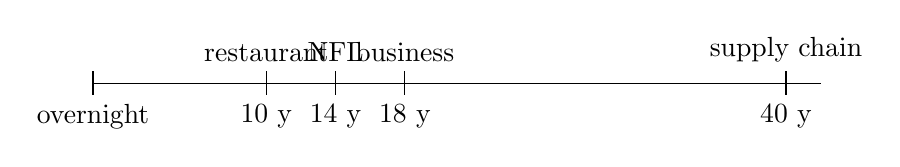
\begin{tikzpicture}[x=0.22cm,y=1cm]
\draw (0,0) -- (42,0);
\draw (0,0.15) -- (0,-0.15);
\node[below] at (0,-0.15) {overnight};
\foreach \x/\top/\bot in {10/restaurant/{10 y},14/NFL/{14 y},18/business/{18 y},40/supply chain/{40 y}} {
  \draw (\x,0.15)--(\x,-0.15);
  \node[above] at (\x,0.15) {\top};
  \node[below] at (\x,-0.15) {\bot};
}
\end{tikzpicture}
\caption{An editorial timeline of the horizons named in the lecture. The attack on ``overnight'' wealth is made concrete by careers measured in decades.}
\end{figure}

The speaker then tells us why this matters. People see images on social media, do not know the truth of other people's situations, and infer that they too must live that way. Thus the lecture's argument against speed is also an argument against imitation. The middle class, in this formulation, is trapped not merely by insufficient income, but by a bad model of what money is for.

\subsection{Question \& Answer}

\paragraph{Question.}
Why does wealth not arrive overnight?

\paragraph{Answer.}
Because the lecture's sequence is not
\[
\text{visibility} \longrightarrow \text{wealth},
\]
but rather
\[
\text{learning} \longrightarrow \text{execution} \longrightarrow \text{scale}.
\]
One must learn from somebody who has actually done the work, accept that the learning phase will not pay like the mature phase, and only then convert borrowed knowledge into independent action. The host's recap immediately after the interview is therefore crucial: find experts, learn everything you can, and then apply and execute. Great things, we are told, take time and sacrifice.

\section{Rock Bottom, Faith, and the Growth Path}

The restaurant-owner interview deepens the lecture by giving us a more complete arc from deprivation to visible scale. Here we are told not only that the speaker has been broke, but that he used to sleep in parking lots. The lecture does not leave that line as an anecdotal flourish. It uses it to motivate a different relation to risk.

\begin{align}
T_{\mathrm{restaurant}} &\approx 10\,\text{years},\\
Y_{\max}^{\mathrm{restaurant}} &\approx \$10\,\text{million},\\
N_{\mathrm{loc}} &= 5,\\
N_{\mathrm{emp}} &\in [85,100].
\end{align}

The turning-point question is answered in a revealing way. Being broke changes what one thinks one can lose. If one is already, in the speaker's words, ``in the ground,'' then trying no longer carries the same terror. The lecture does not formalize this as expected utility, but it does narrate a shift in decision geometry: the downside has already been visited, and so motion becomes easier.

\subsection{Question \& Answer}

\paragraph{Question.}
What is an actionable step when somebody is at rock bottom?

\paragraph{Answer.}
The answer in this interview is explicit and should not be diluted: one must put God in the heart. The speaker presents this not as a decorative sentiment, but as the first practical reordering of life. From there the instruction is simple: go forward, push hard, and continue. The lecture is therefore careful here. It does not offer a generic motivational algorithm. It preserves the speaker's own causal account of recovery.

The scaling portion of the interview is equally important. We begin inside a gas station with what sounds like a two-person operation: the owner and one additional worker. We end with multiple locations and a staff in the high double digits.

\paragraph{Worked scaling example.}
If we take ``me and one guy'' literally, the transcript suggests the rough growth path
\begin{align}
N_{\mathrm{loc}} &: 1 \to 5,\\
N_{\mathrm{emp}} &: 2 \to [85,100].
\end{align}
Hence the implied scale multiples are
\begin{equation}
\frac{N_{\mathrm{loc,final}}}{N_{\mathrm{loc,initial}}} = 5,
\qquad
\frac{N_{\mathrm{emp,final}}}{N_{\mathrm{emp,initial}}} \in [42.5,50].
\end{equation}

This is only an editorial compression of the spoken narrative, not a full business model. Still, it captures something the lecture wants us to see: the move from a tiny starting point to a visibly staffed, multi-location operation is not rhetorical. It is operational.

The interview then turns to education. The speaker's complaint is not simply anti-school. It is more precise. If the aim is business, then instruction without lived business experience can feel detached from the thing it claims to teach. The recommended alternative is apprenticeship: wake up early, stand on the business side, and keep working regardless of how much money or how many businesses one already has.

\section{Interruption, Saving Bread, and Long Careers}

At this point the lecture is interrupted by security. This is not dead space. The interruption forces the host to restate the mission of the channel and to place risk into the argument itself: take the risk or lose the chance. The lecture then resumes with renewed momentum and turns to the most public figure in the chapter, Von Miller.

The athlete interview makes the next decisive move. Up to now we have mostly discussed how wealth is built. Now we are asked how wealth is preserved. The answer is compressed into a repeated phrase: save bread.

\begin{align}
Y_{\max}^{\mathrm{NFL}} &= \$38\,\text{million},\\
T_{\mathrm{NFL}} &\approx 14\,\text{years}.
\end{align}

The lecture never writes a board equation here, but the verbal structure is clear enough that we can state the bookkeeping identity behind it.

\paragraph{A minimal update rule.}
Let \(Y_t\) be income in period \(t\), \(C_t\) consumption, \(S_t\) retained savings, \(W_t\) wealth stock, and \(R_t\) the return generated by already retained capital. Then
\begin{align}
S_t &= Y_t - C_t,\\
W_{t+1} &= W_t + S_t + R_t.
\end{align}
Subtracting \(W_t\) from both sides gives the update rule
\begin{align}
\Delta W_t &= W_{t+1} - W_t \\
&= Y_t - C_t + R_t.
\end{align}

This is the right place to hear the repeated phrase ``save bread.'' The lecture's point is not that high income automatically implies growing wealth. Quite the opposite. If \(C_t\) rises until it nearly absorbs \(Y_t\), then \(S_t\) collapses, and the wealth stock no longer grows by retained income. That is why the host immediately invokes stories of elite earners who went broke. The athlete's advice is concise precisely because the arithmetic underneath it is not complicated: earning is not enough if one does not retain.

A short example makes the point. If a person earns an extraordinary annual income \(Y_t\) but spends nearly all of it, so that \(C_t \approx Y_t\), then \(S_t \approx 0\), and the update rule becomes approximately
\[
\Delta W_t \approx R_t.
\]
In that case the large income has done very little by itself. Wealth persists only if retained income and later returns are allowed to work.

The lecture then broadens from financial retention to personal durability. Miller answers the question of competitive separation with resilience and the ability to evolve. He answers the question of longevity with a mixture of grace, bodily preparation, mental health, and self-awareness. Thus long career life is treated as another form of preservation problem. One must preserve not only money, but also the human instrument that produces it.

\section{Risk, Sacrifice, and the Final Interview}

The final substantial interview returns us to a smaller scale of income but not to a smaller scale of principle. We are again given an eighteen-year business horizon, a reported peak annual income of half a million dollars, and another memory of not having enough food. But the emphasis now falls on early risk and on the refusal to remain content with a safe paycheck.

\begin{align}
T_{\mathrm{business}} &\approx 18\,\text{years},\\
Y_{\max}^{\mathrm{final}} &= \$500{,}000.
\end{align}

The lecture's logic here is cumulative. Earlier we learned that truth supports business, that patience defeats the fantasy of instant wealth, that rock bottom can alter the relation to risk, and that retained income matters more than raw income. The final interview gathers these lines together. The speaker says that one does not meet one's full potential without taking risks early, and that the biggest risk in his own career was stepping out independently rather than working hard merely so that a larger company could succeed.

The closing answer to the question of becoming a millionaire in 2024 is correspondingly composite. Be willing to make sacrifices. Work hard. Do not show off. Be honest. Do not be afraid to reach out to people and ask for advice or support. The lecture ends, then, not with a secret tactic but with a combination of moral, temporal, and relational disciplines.

\section{Summary}

The chapter begins with visible wealth and ends with a more exact account of what sustains it. The sequence is deliberate. First we are taught that business rests on truth and credibility. Then we are taught that wealth takes time, that imitation is a trap, and that apprenticeship matters. Then we are shown how poverty changes the meaning of risk and how small operations can scale. After that the lecture turns to preservation: saving, restraint, resilience, health, and long duration. Finally it closes by returning to sacrifice, honesty, and the willingness to step out on one's own.

If we compress the whole lecture into one line, it is this: large outcomes are real, but they are not the first thing. The first thing is the mechanism that keeps them from dissolving.